\newsection
\section{Технический проект}
\subsection{Общая характеристика организации решения задачи}

Планирование и создание веб-сайта необходимо для того, чтобы оптимизировать способ хранения и организации информации в медицинской лаборатории.

Веб-сайт - это набор веб-страниц, размещенных на сервере и связанных между собой. Каждая веб-страница содержит информацию, которая может быть представлена в различных форматах, таких как текст, изображения и видео, среди прочих. Эти веб-сайты создаются с определенной целью, будь то информирование, продвижение товаров или услуг, предоставление развлечений и т.д. Создание веб-сайта включает в себя планирование, проектирование и разработку логической структуры для представления информации в Интернете с целью облегчения доступа и удобства для пользователей\cite{website}.

Веб-сайт может иметь и другие элементы, такие как контактные формы, системы внутреннего поиска, ссылки на другие веб-сайты, кнопки для обмена контентом в социальных сетях, а также другие элементы, направленные на улучшение производительности и функциональности сайта.

Существуют также различные типы веб-сайтов, от личных страниц и блогов до интернет-магазинов и корпоративных сайтов. Каждый тип веб-сайта имеет свои специфические характеристики и цели.

Процесс создания веб-сайта включает в себя выбор платформы или языка программирования, выбор веб-хоста, приобретение доменного имени, создание контента и графического дизайна. Также важно учитывать использование методов SEO (поисковой оптимизации), чтобы сделать сайт видимым в результатах поиска поисковых систем.

Общая организация веб-сайта медицинской лаборатории зависит от конкретного содержания, которое вы хотите представить, и цели, которую вы хотите достичь. Ниже перечислены некоторые разделы веб-сайта медицинской лаборатории:

\begin{enumerate}
	\item Главная страница: страница приветствия, на которой есть поля для входа в систему и ввода пароля врача.
	\item Услуги: навигационный раздел, в котором перечислены предлагаемые услуги, такие как анализы крови, медицинские анализы и другие медицинские услуги.
	\item Формы: раздел для заполнения личных данных пациента, а также записей о его лечении, наблюдении, приеме лекарств и анализах с помощью формы с обязательными и необязательными полями.
	\item Результаты: раздел, в котором врачи могут получить доступ к результатам лабораторных анализов в режиме онлайн в безопасной и эффективной системе.
	\item Навигационные таблицы: включает навигационную таблицу для поиска ранее зарегистрированных пациентов.
\end{enumerate}

медицинская лаборатория уникальна, поэтому разделы продумываются исходя из конкретных целей и потребностей. Сайт интуитивно понятен и предлагает клиницисту оптимальную навигацию для поиска актуальной и полезной информации о пациенте.

\subsubsection{Словарь предметной области продукта веб-странице изделия}

Тщательный анализ предметной области был проведен в технической спецификации, а термины на английском и испанском языках были собраны в словаре по предметной области. Этот словарь основан на разделе № 2 технической спецификации. С другой стороны, в таблице \ref{table:dic} представлен словарь данных среды разрабатываемой веб-страницы, отвечающий за выполнение всех услуг, предлагаемых веб-страницей для медицинской лаборатории.


\begin{xltabular}{\textwidth}{|p{4cm}|p{12cm}|}
	\caption{Словарь данных для части среды разрабатываемой веб-страницы.\label{table:dic}}\\ \hline
	\thead{Термин} & \thead{Описание} \\ \hline
	\thead{1} & \thead{2} \\ \hline
	\endfirsthead
	\continuecaption{Продолжение таблицы \ref{table:dic}}
	\thead{1} & \thead{2} \\ \hline
	\finishhead
	Поле«интерфейс входа в систему» & Это главная страница, на которой будут подтверждены логин и пароль врача \\ \hline 
	Поле«форма для пациентов» & После подтверждения имени пользователя и пароля, введенного непосредственно в форму для регистрации нового пациента, здесь пользователь должен заполнить поля в форуме, если он хочет ввести нового пациента. \\ \hline 
	Поле«специальная форма» & В зависимости от специальности, выбранной врачом или медсестрой, будет развернута форма специальности.  \\ \hline 
	Поле«форма нового врача» & Пользователь сможет ввести личные данные нового врача, который будет работать в медицинской лаборатории, и указать имя пользователя и пароль.  \\ \hline 
	Поле«информация о пациентах» & Врач или медсестра смогут просмотреть в таблице все данные о пациентах, поступивших в медицинскую лабораторию. \\ \hline 
	Поле«выход из системы» & При заполнении этого поля система закроет начатый сеанс врача.  \\ \hline 
\end{xltabular}

\subsection{Обоснование выбора технологии проектирования}

Использование веб-сайта в медицинской лаборатории оправдано по нескольким причинам. Веб-сайт поможет улучшить организацию и учет информации, облегчая доступ к данным в режиме онлайн. Он также может служить платформой для передачи соответствующей информации врачам. Кроме того, веб-сайт обеспечивает безопасность только для сотрудников, обученных работе с личной информацией пациентов, проведенными тестами, лечением и результатами. Веб-сайт также может использоваться для регистрации данных о врачах с указанием их специальностей и номеров кабинетов, где они находятся.

В настоящее время длительные процессы можно решить с помощью собственного программного обеспечения, поскольку хорошая поддержка мультимедиа HTML способна легко интегрировать мультимедийные элементы, такие как изображения, видео и аудио, в веб-страницу, что выгодно, когда вы хотите обеспечить разнообразие в контенте.

Гибкость дизайна HTML как языка разметки позволяет дизайнерам создавать индивидуальные стили и макеты страниц, предоставляя разработчикам полный контроль над визуальным оформлением веб-страниц.

\subsubsection{Описание используемых технологий и языков программирования}

При создании веб-сайта используются различные программные инструменты и языки программирования, каждый из которых применяется в зависимости от различных задач, которые необходимо выполнить.

HTML - одна из основополагающих технологий в веб-программировании. HTML используется для определения структуры и содержания веб-страницы, то есть элементов, из которых она состоит, и их иерархической организации.
В дополнение к HTML существуют и другие технологии, такие как CSS, которые позволяют определять стили и визуальное форматирование веб-страницы.
HTML был разработан в начале 1990-х годов и с течением времени развивался, включая новые функции и возможности. Совет Всемирной паутины (W3C) является организацией, ответственной за разработку и поддержание стандартов HTML.
Навыки, необходимые для изучения HTML, включают понимание тегов, базовой структуры веб-страниц, атрибутов, ссылок, форм, а также использование изображений и видео.
В целом, HTML - это важный язык разметки, используемый для разработки современных веб-страниц и являющийся фундаментальным компонентом веб-программирования.
HTML используется для создания структурированного веб-контента. 
HTML-теги позволяют организовать содержимое веб-страницы в различные разделы, такие как заголовки, абзацы, таблицы, изображения, формы и ссылки. медицинские лаборатории могут использовать эти теги, чтобы сделать свою информацию легко читаемой и доступной для клиницистов.
Оформление и внешний вид веб-сайта также должны соответствовать медицинскому имиджу лаборатории. Поэтому была использована соответствующая цветовая схема и обеспечено профессиональное и четкое представление контента.

\subsubsection{Язык программирования PHP}

PHP использовался на сайте для разработки системы управления пациентами, в которой хранится информация о пациентах и упорядочивается администрирование и организация медицинских услуг лаборатории. Он также использовался для автоматизации обработки и анализа медицинских данных, создания отчетов и интеграции с другими медицинскими информационными системами. PHP способен взаимодействовать с базами данных, что выгодно для записи, запроса и поиска информации быстро и эффективно\cite{php2}.
PHP имеет такие фреймворки, как Laravel и Symfony, которые делают его очень мощным и профессиональным. Важно отметить, что PHP является объектно-ориентированным языком, что позволяет использовать его для решения множества задач программирования. Он также имеет большое сообщество, что гарантирует постоянную поддержку и регулярные обновления языка\cite{php1}. 

PHP имеет C-подобный синтаксис и предназначен для взаимодействия с базами данных и доставки динамического содержимого через Интернет с помощью технологии веб-сервера. Некоторые из наиболее заметных особенностей PHP следующие:

\begin{enumerate}
	\item Интерпретация: исходный код PHP выполняется на сервере перед отправкой страницы в браузер пользователя.
	\item Простая интеграция с HTML: PHP позволяет внедрять PHP-код внутрь HTML-страниц для создания динамических веб-страниц.
	\item Подключение к базе данных: PHP имеет широкий спектр расширений для подключения к базам данных, что облегчает разработку приложений, использующих базы данных.
	\item Объектно-ориентированный: PHP также поддерживает объектно-ориентированное программирование.
	\item Обширная документация и сообщество: PHP имеет обширную документацию и активное онлайн-сообщество пользователей, которые предлагают поддержку и ресурсы для разработки на этой технологии.
\end{enumerate}

PHP работает на сервере и генерирует HTML, который отправляется в браузер пользователя для отображения. Помимо HTML, PHP может генери ровать и другие типы контента, такие как изображения и PDF-файлы.
Использование PHP на сайте медицинской лаборатории полезно, поскольку это язык программирования, позволяющий создавать динамический контент на сайте. PHP использовался для создания интерактивных форм, автоматизации онлайн-задач, интеграции баз данных и защиты информации о пациентах.
В медицинской лаборатории PHP может быть использован для создания страницы с интерактивными формами, позволяющими врачам регистрироваться и получать информацию в автоматическом режиме.
PHP имеет множество функций безопасности для защиты целостности данных пациентов, что делает его хорошим выбором для медицинской среды.

\subsubsection{Преимущества языка PHP}

Существует несколько преимуществ использования PHP для разработки веб-сайта, например, следующие:

\begin{enumerate}
	\item Легкость изучения: PHP считается одним из самых простых языков для изучения, что делает его популярным среди начинающих разработчиков.
	\item Доступность на различных платформах: PHP работает на различных операционных системах, что делает его гибким и универсальным.
	\item Интеграция с MySQL: Используя PHP в сочетании с MySQL, вы получаете доступ к широким возможностям работы с данными и их обработки.
	\item Большое и опытное сообщество: Существует большое сообщество разработчиков и пользователей PHP по всему миру, которые делятся своими знаниями и ресурсами, что облегчает процесс обучения и устранения неполадок.
	\item Скорость выполнения: PHP предлагает быстрое и эффективное выполнение по сравнению с другими языками программирования.
	\item Персонализация: PHP очень легко настраивается и адаптируется к различным потребностям и специфическим требованиям проектов веб-разработки.
\end{enumerate}

\subsubsection{Недостатки языка PHP}

К недостаткам использования PHP на веб-странице можно отнести следующие:

\begin{enumerate}
	\item Проблемы безопасности: При неправильной настройке использование PHP на веб-странице может вызвать проблемы с безопасностью, поскольку этот язык позволяет выполнять код на сервере.
	\item Необходимость в веб-сервере: Для того чтобы веб-страница могла выполнять код PHP, требуется веб-сервер, что может увеличить расходы на хостинг и обслуживание.
	\item Ограниченная масштабируемость: По мере роста и усложнения веб-сайта производительность PHP может быть ограничена.
	\item Сложная отладка: При работе с PHP-кодом может быть трудно отлаживать специфические ошибки и проблемы из-за сложности языка.
	\item Избыточный код: PHP может генерировать громоздкий код на веб-страницах, что может замедлить скорость загрузки и негативно повлиять на пользовательское восприятие.
\end{enumerate}

\subsection{Язык стилей CSS}

Использование CSS на сайте медицинской лаборатории определило визуальное представление и стиль сайта, что помогает улучшить опыт врача и облегчает понимание информации, представленной на сайте. В целом, CSS помогает улучшить представление и читабельность информации на странице, что может быть полезно в условиях, когда важно представить медицинскую информацию четко и точно.

Таблицы стилей CSS содержат правила, определяющие стиль элементов HTML, к которым они применяются\cite{css1}. Каждое правило состоит из селектора, указывающего элементы, к которым будет применен стиль, и набора свойств, определяющих стиль элемента. Свойства могут включать цвет фона, шрифт, размер шрифта, межстрочный интервал, размер границы и другие.

\subsubsection{Достоинства языка CSS}

К преимуществам языка стилей CSS относятся:

\begin{enumerate}
	\item Разделение содержания и представления, что облегчает обслуживание и модификацию сайта.
	\item Эффективность загрузки страницы, поскольку стили могут быть определены и применены к различным элементам.
	\item Гибкость дизайна, поскольку настраиваемые стили могут применяться и адаптироваться к различным устройствам и разрешениям.
	\item Простота использования, поскольку это декларативный язык, а его синтаксис интуитивно понятен и прост для понимания.
	\item Он позволяет создавать целостный дизайн всего сайта, что повышает удобство использования и улучшает впечатления пользователей.
\end{enumerate}

\subsubsection{Недостатки языка CSS}

К возможным недостаткам языка стилей CSS относятся следующие:
\begin{enumerate}
	\item Сложность обучения правильному использованию, особенно для дизайнеров, которые привыкли использовать графические инструменты для создания дизайна.
	\item Возможна несовместимость между различными браузерами и версиями, что может потребовать дополнительного тестирования и корректировки стилей для обеспечения совместимости.
	\item Поскольку это универсальный и гибкий инструмент, могут возникнуть проблемы с производительностью, если применяется слишком много сложных стилей или они не оптимизированы должным образом.
	\item Для выполнения некоторых сложных задач CSS могут потребоваться дополнительные навыки программирования.
\end{enumerate}

В целом, однако, преимущества CSS значительно превосходят потенциальные недостатки, и он зарекомендовал себя как ключевой элемент эффективного дизайна современных веб-сайтов.

\subsection{Диаграмма компонентов и схема обмена данными между файлами компонента}

Диаграммы компонентов полезны в программировании, поскольку они дают общее представление о системе и определяют взаимосвязи между различными компонентами, что облегчает понимание и сопровождение кода и может помочь выявить потенциальные проблемы и улучшения в системе. Кроме того, диаграммы компонентов могут служить основой для построения архитектуры программного обеспечения и планирования его развития.

На рисунке \ref{image:diagram} показана компонентная диаграмма работы сайта.

\begin{figure}
\centering{\includegraphics[width=1\linewidth]{diagramadecomponentes}}
\caption{Диаграмма компонентов}
\label{image:diagram}
\end{figure}

Вызов любого компонента на веб-странице требует, чтобы он был включен в код сценария соответствующей страницы. При вызове компонента происходит передача данных от страницы к соответствующему компоненту.

На рисунке \ref{image:diagram2} показано, как происходит обмен данными между скриптами компонента и веб-страницей при вызове компонента.

\begin{figure}
\centering{\includegraphics[width=0.5\linewidth]{diagramacomp2}}
\caption{Схема обмена данными между веб-страницей и скриптом}
\label{image:diagram2}
\end{figure}

Сценарий веб-страницы устанавливает значения параметров компонента во время вызова, которые затем передаются сценарию в файле index.php.
В скрипте файла index.php метод session\_stat с помощью метода\linebreak if(isset(isset(\$SEASION['user\_id']))) вызывает компонент login.php, в котором будет проверен пользователь, желающий войти на платформу сайта. Идентификатор врача будет авторизован для доступа ко всем функциям сайта.\linebreak После эффективного входа подключается скрипт файла Patient.php одного из шаблонов, который представлен формой для регистрации персональных данных каждого пациента. С помощью компонента nav.html врач может выбрать варианты навигационного меню сайта. Если в меню будет выбран пункт ``Doctors'', то будет вызван скрипт doctors.php - шаблон, в котором будет отображена форма для ввода персональных данных врачей, работающих в медицинской лаборатории. Аналогично, если будет выбран пункт ``Analysis'', то будет вызван скрипт каждой нужной специальности и отображена форма для регистрации каждого пациента по специальности. 

Операции скрипта и все, что зарегистрировано из форм, вызовут метод Conexion.php, который осуществит соединение с базой данных, и произведет консультацию, сохранение и удаление информации в базе данных.

\subsection{Диаграмма развертывания}

Диаграмма размещения (рис.~\ref{image:diagram3}) представляет физические взаимодействия, существующие между аппаратными и программными частями анализируемой системы.

\begin{figure}
\centering{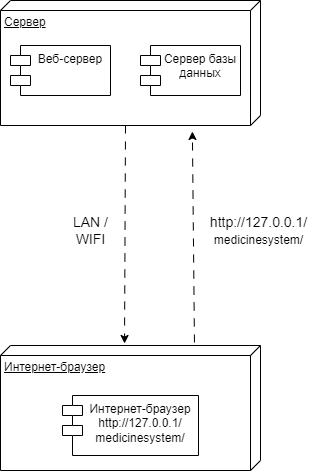
\includegraphics[width=0.37\linewidth]{diagramacomp3}}
\caption{Диаграмма развертывания}
\label{image:diagram3}
\end{figure}

Диаграмма размещения показывает представление физических взаимодействий между аппаратными и программными частями системы веб-сайта с серверами.

\subsection{Схема базы данных}

Диаграммы таблиц MySQL - полезный инструмент для визуализации структуры базы данных и связей между ее таблицами, поскольку они облегчают понимание структуры базы данных. Представление базы данных MySQL покажет реализацию и архитектуру таблиц для данных о специальности, враче и пациенте медицинской лаборатории.
Диаграмма на \ref{image:base} показывает мертвые таблицы, созданные в MySQL.

База данных может быть полезна для управления данными в медицинской лаборатории. медицинские лаборатории производят большое количество данных о пациентах, включая информацию о лабораторных тестах и другую медицинскую информацию. База данных в медицинской лаборатории включает в себя:

\begin{enumerate}
	\item Хранение информации о пациенте и истории болезни.
	\item Хранение информации о проведенных лабораторных тестах и полученных результатах.
	\item Выявление закономерностей в данных для идентификации типов пациентов и результатов лабораторных тестов.
	\item Формирование отчетов о результатах лабораторных исследований для обеспечения лечения пациента.
	\item Повышение качества данных и сокращение количества ошибок путем проверки данных и выявления ошибок перед сохранением данных в базе данных.
\end{enumerate}

\begin{figure}
	\centering{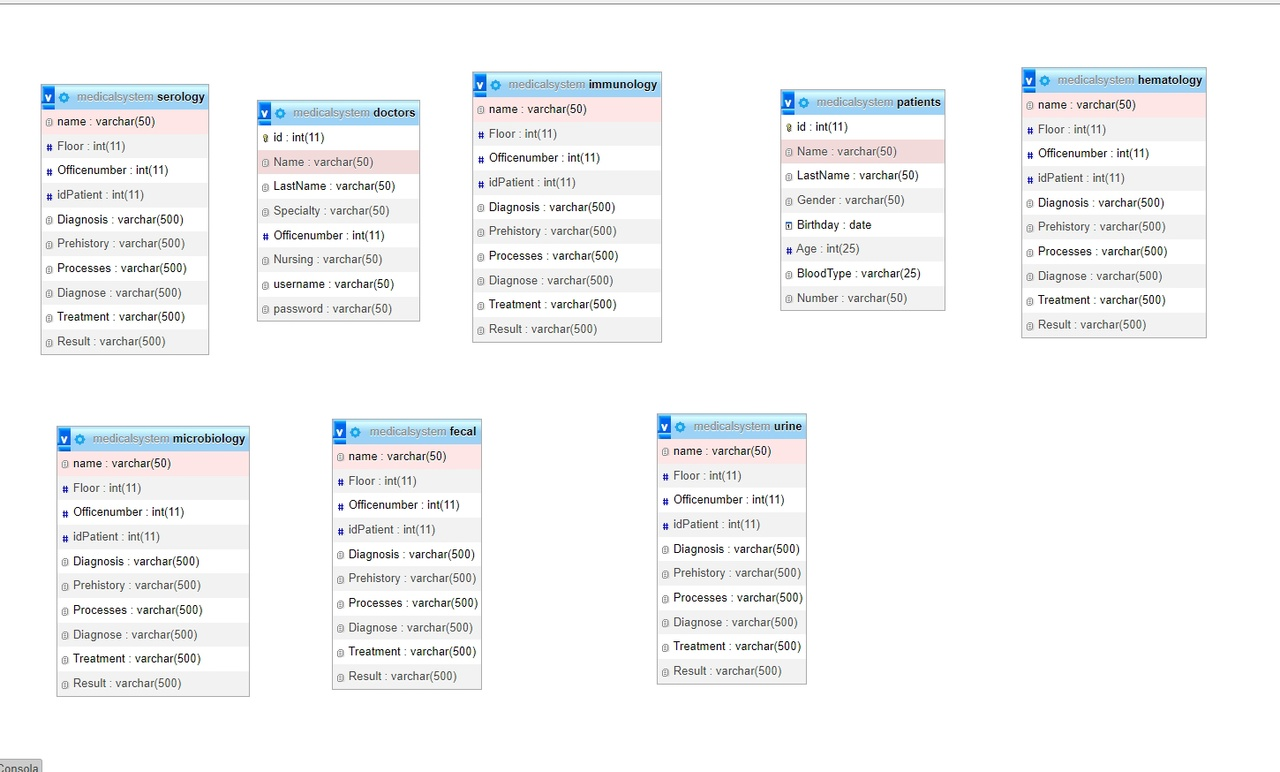
\includegraphics[width=1\linewidth]{base}}
	\caption{Схема базы данных}
	\label{image:base}
\end{figure}

\subsection{Содержание форм на веб-сайте}

Веб-сайт медицинской лаборатории играет ключевую роль в общении с врачами, предоставляя важную информацию о предоставляемых услугах и результатах. Одним из наиболее важных аспектов веб-сайта медицинской лаборатории является содержание форм, представленных на сайте. Эти формы должны быть четкими, полными и эффективными, чтобы обеспечить удовлетворительный опыт для врачей.

Во-первых, онлайн-формы легко найти и выбрать на сайте медицинской лаборатории, а четкая и интуитивно понятная структура позволяет врачам быстро найти и заполнить формы. Кроме того, формы адаптируемы, так что их можно читать и заполнять на любом компьютере, без потери качества и удобства использования.

Во-вторых, бланки имеют хорошую организацию и структуру, с четкими инструкциями по каждому из разделов. 

В-третьих, бланки медицинской лаборатории безопасны. Пациенты должны быть уверены, что информация, которую они предоставляют в бланках, будет обрабатываться конфиденциально и безопасно. На сайте предусмотрены адекватные меры безопасности для защиты личной и медицинской информации, собранной в бланках.

Наконец, важно, чтобы лаборатория постоянно обновляла бланки, предоставляя последнюю информацию о выполненных для пациентов услугах, обеспечивая точность и актуальность бланков для врачей.

Формы на сайте, состоящие из обязательных и необязательных полей, основаны на следующих трех структурах:

\begin{itemize}
\item "<Doctors">;
\item "<Patient">;
\item "<Analysis">.
\end{itemize}

В форме "<Doctors"> содержит поля, показанные в следующей таблице \ref{table:doctors}.

\begin{xltabular}{\textwidth}{|l|l|p{1.7cm}|X|}
	\caption{Форме "<Doctors">\label{table:doctors}}\\ \hline
	\thead{Поле} & \thead{Тип} & \thead{Обяза-\\тельное} & \thead{Описание} \\ \hline
	\thead{1} & \thead{2} & \thead{3} & \thead{4} \\ \hline
	\endfirsthead
	\continuecaption{Продолжение таблицы \ref{table:doctors}}
	\thead{1} & \thead{2} & \thead{3} & \thead{4} \\ \hline
	\finishhead
	id & int & true & Идентификатор врача \\ \hline 
	Name & varchar(50) & true & Имя врача \\ \hline 
	LastName & varchar(50) & true & Фамилия врача \\ \hline 
	Specialty & varchar(50) & true & Специальность врача \\ \hline 
	Officenumber & int & false & Офис, где работает врач \\ \hline 
	Nursing & varchar(50) & true & ФИО медсестры \\ \hline 
	username & varchar(50) & true & Пользователь для входа в систему \\ \hline
	password & varchar(50) & true & Пароль врача для входа в систему \\ \hline
\end{xltabular}

Для формы "<Patient"> поля описаны в следующей таблице \ref{table:patient}.


\begin{xltabular}{\textwidth}{|l|l|p{1.7cm}|X|}
	\caption{Форме "<Patient">\label{table:patient}}\\ \hline
	\thead{Поле} & \thead{Тип} & \thead{Обяза-\\тельное} & \thead{Описание} \\ \hline
	\thead{1} & \thead{2} & \thead{3} & \thead{4} \\ \hline
	\endfirsthead
	\continuecaption{Продолжение таблицы \ref{table:patient}}
	\thead{1} & \thead{2} & \thead{3} & \thead{4} \\ \hline
	\finishhead
	id & int & true & Идентификатор пациента \\ \hline 
	Name & varchar(50) & true & Имя пациента \\ \hline 
	LastName & varchar(50) & true & Фамилия пациента \\ \hline 
	Gender & varchar(50) & true & Пол пациента \\ \hline 
	Birthday & date & true & Дата рождения пациента \\ \hline 
	Age & int & true & Возраст пациента \\ \hline 
	BloodType & varchar(25) & true & Определение группы крови пациента \\ \hline
	Number & varchar(50) & false & Контактный номер пациента \\ \hline
\end{xltabular}

В форме "<Analysis"> одна и та же форма используется для всех специальностей медицинской лаборатории и содержит поля, показанные в следующей таблице\ref{table:anali}.

\begin{xltabular}{\textwidth}{|l|l|p{1.7cm}|X|}
	\caption{Форме "<Analysis">\label{table:anali}}\\ \hline
	\thead{Поле} & \thead{Тип} & \thead{Обяза-\\тельное} & \thead{Описание} \\ \hline
	\thead{1} & \thead{2} & \thead{3} & \thead{4} \\ \hline
	\endfirsthead
	\continuecaption{Продолжение таблицы \ref{table:anali}}
	\thead{1} & \thead{2} & \thead{3} & \thead{4} \\ \hline
	\finishhead
	name & varchar(50) & true & ФИО врача-специалиста \\ \hline 
	Floor & int & false & Этаж здания, где находится специальность \\ \hline 
	idPatient & int & true & ФИО пациента \\ \hline 
	Diagnosis & varchar(500) & true & Диагноз пациента \\ \hline 
	Prehistory & varchar(500) & true & История болезни пациента \\ \hline 
	Processes & varchar(500) & true & Процедуры, проводимые с пациентом \\ \hline 
	Diagnose & varchar(500) & true & Текущий диагноз пациента \\ \hline
	Treatment & varchar(500) & true & Лечение пациента \\ \hline
	Result & varchar(500) & true & Результат процессов, проведенных с пациентом \\ \hline
\end{xltabular}

В большинство полей формы ``Analysis'' разрешается вводить текст объемом до 500 символов. История болезни каждого пациента будет уникальна и будет связана с именем пациента, а также с врачом, который проводил процессы у пациента.
Разработанная база данных помогает медицинской лаборатории эффективно хранить, организовывать и управлять данными о пациентах и аналитическими данными, что способствует повышению качества ее данных и созданию точных и полезных отчетов.

\subsection{Моделирование прецедентов}

Для моделирования вариантов использования веб-страницы для медицинской лаборатории в качестве важной части процесса разработки были предоставлены варианты использования, которые помогают определить требования и функциональные возможности веб-страницы и позволяют понять, как пользователи будут взаимодействовать со страницей.

Чтобы смоделировать варианты использования веб-страницы, были предприняты следующие шаги:

\begin{enumerate}
	\item Определение требований: на этом первом этапе были определены необходимые требования, которым должен соответствовать веб-сайт медицинской лаборатории. Это включало понимание потребностей и ожиданий конечного пользователя.
	\item Идентификация субъектов: были определены основные субъекты, которые будут взаимодействовать с веб-страницей, что помогло определить объем и сложность вариантов использования.
	\item Идентификация вариантов использования: на основе выявленных требований и действующих лиц можно было определить необходимые варианты использования для веб-страницы. Эти варианты использования включали такие задачи, как регистрация пациентов, регистрация врачей, регистрация анализов и просмотр результатов тестов.
\end{enumerate}

Описание функций, используемых системой на веб-сайте.
Работа системы состоит из трех основных функций. Эти характеристики описаны ниже.
Имя функции: session\_start();
Предварительное условие: ввод действительных данных пользователя и пароля.
Последующее условие: вызывает функцию Connection, в которой пользователь проверяется на соответствие данным, записанным в базе данных.
Описание функции session\_start(): эта функция при вызове подключения к базе данных проверяет имя пользователя и пароль с данными врачей в базе данных.

Название функции: подключение.
Предварительное условие: система автоматически вводит данные с веб-страницы.
Последующее условие: система ищет таблицу формулы, выбранной пользователем.
Описание функции подключение: это линия подключения к базе данных и таблицам для соответствующей записи введенных данных о новых врачах, пациентах и специальностях по выбору пользователя.

Название функции: сохранить.
Предварительное условие: пользователь заполняет поля используемой формы.
Последующее условие: система записывает то, что было введено через поля шаблона.
Описание функции сохранения: функция выполняет проверку достоверной информации в соответствии с правилами, содержащимися в каждой таблице базы данных, чтобы продолжить соответствующую регистрацию и сохранение введенного пользователем.